% Options for packages loaded elsewhere
\PassOptionsToPackage{unicode}{hyperref}
\PassOptionsToPackage{hyphens}{url}
%
\documentclass[
  14pt,
  a5paper,
]{extarticle}
\usepackage{amsmath,amssymb}
\usepackage{iftex}
\ifPDFTeX
  \usepackage[T1]{fontenc}
  \usepackage[utf8]{inputenc}
  \usepackage{textcomp} % provide euro and other symbols
\else % if luatex or xetex
  \usepackage{unicode-math} % this also loads fontspec
  \defaultfontfeatures{Scale=MatchLowercase}
  \defaultfontfeatures[\rmfamily]{Ligatures=TeX,Scale=1}
\fi
\usepackage{lmodern}
\ifPDFTeX\else
  % xetex/luatex font selection
  \setmainfont[]{Noto Sans CJK JP}
  \setsansfont[]{Noto Sans CJK JP}
  \setmonofont[]{Noto Sans Mono CJK JP}
\fi
% Use upquote if available, for straight quotes in verbatim environments
\IfFileExists{upquote.sty}{\usepackage{upquote}}{}
\IfFileExists{microtype.sty}{% use microtype if available
  \usepackage[]{microtype}
  \UseMicrotypeSet[protrusion]{basicmath} % disable protrusion for tt fonts
}{}
\makeatletter
\@ifundefined{KOMAClassName}{% if non-KOMA class
  \IfFileExists{parskip.sty}{%
    \usepackage{parskip}
  }{% else
    \setlength{\parindent}{0pt}
    \setlength{\parskip}{6pt plus 2pt minus 1pt}}
}{% if KOMA class
  \KOMAoptions{parskip=half}}
\makeatother
\usepackage{xcolor}
\usepackage[margin=12mm]{geometry}
\usepackage{color}
\usepackage{fancyvrb}
\newcommand{\VerbBar}{|}
\newcommand{\VERB}{\Verb[commandchars=\\\{\}]}
\DefineVerbatimEnvironment{Highlighting}{Verbatim}{commandchars=\\\{\}}
% Add ',fontsize=\small' for more characters per line
\newenvironment{Shaded}{}{}
\newcommand{\AlertTok}[1]{\textcolor[rgb]{1.00,0.00,0.00}{\textbf{#1}}}
\newcommand{\AnnotationTok}[1]{\textcolor[rgb]{0.38,0.63,0.69}{\textbf{\textit{#1}}}}
\newcommand{\AttributeTok}[1]{\textcolor[rgb]{0.49,0.56,0.16}{#1}}
\newcommand{\BaseNTok}[1]{\textcolor[rgb]{0.25,0.63,0.44}{#1}}
\newcommand{\BuiltInTok}[1]{\textcolor[rgb]{0.00,0.50,0.00}{#1}}
\newcommand{\CharTok}[1]{\textcolor[rgb]{0.25,0.44,0.63}{#1}}
\newcommand{\CommentTok}[1]{\textcolor[rgb]{0.38,0.63,0.69}{\textit{#1}}}
\newcommand{\CommentVarTok}[1]{\textcolor[rgb]{0.38,0.63,0.69}{\textbf{\textit{#1}}}}
\newcommand{\ConstantTok}[1]{\textcolor[rgb]{0.53,0.00,0.00}{#1}}
\newcommand{\ControlFlowTok}[1]{\textcolor[rgb]{0.00,0.44,0.13}{\textbf{#1}}}
\newcommand{\DataTypeTok}[1]{\textcolor[rgb]{0.56,0.13,0.00}{#1}}
\newcommand{\DecValTok}[1]{\textcolor[rgb]{0.25,0.63,0.44}{#1}}
\newcommand{\DocumentationTok}[1]{\textcolor[rgb]{0.73,0.13,0.13}{\textit{#1}}}
\newcommand{\ErrorTok}[1]{\textcolor[rgb]{1.00,0.00,0.00}{\textbf{#1}}}
\newcommand{\ExtensionTok}[1]{#1}
\newcommand{\FloatTok}[1]{\textcolor[rgb]{0.25,0.63,0.44}{#1}}
\newcommand{\FunctionTok}[1]{\textcolor[rgb]{0.02,0.16,0.49}{#1}}
\newcommand{\ImportTok}[1]{\textcolor[rgb]{0.00,0.50,0.00}{\textbf{#1}}}
\newcommand{\InformationTok}[1]{\textcolor[rgb]{0.38,0.63,0.69}{\textbf{\textit{#1}}}}
\newcommand{\KeywordTok}[1]{\textcolor[rgb]{0.00,0.44,0.13}{\textbf{#1}}}
\newcommand{\NormalTok}[1]{#1}
\newcommand{\OperatorTok}[1]{\textcolor[rgb]{0.40,0.40,0.40}{#1}}
\newcommand{\OtherTok}[1]{\textcolor[rgb]{0.00,0.44,0.13}{#1}}
\newcommand{\PreprocessorTok}[1]{\textcolor[rgb]{0.74,0.48,0.00}{#1}}
\newcommand{\RegionMarkerTok}[1]{#1}
\newcommand{\SpecialCharTok}[1]{\textcolor[rgb]{0.25,0.44,0.63}{#1}}
\newcommand{\SpecialStringTok}[1]{\textcolor[rgb]{0.73,0.40,0.53}{#1}}
\newcommand{\StringTok}[1]{\textcolor[rgb]{0.25,0.44,0.63}{#1}}
\newcommand{\VariableTok}[1]{\textcolor[rgb]{0.10,0.09,0.49}{#1}}
\newcommand{\VerbatimStringTok}[1]{\textcolor[rgb]{0.25,0.44,0.63}{#1}}
\newcommand{\WarningTok}[1]{\textcolor[rgb]{0.38,0.63,0.69}{\textbf{\textit{#1}}}}
\usepackage{longtable,booktabs,array}
\usepackage{calc} % for calculating minipage widths
% Correct order of tables after \paragraph or \subparagraph
\usepackage{etoolbox}
\makeatletter
\patchcmd\longtable{\par}{\if@noskipsec\mbox{}\fi\par}{}{}
\makeatother
% Allow footnotes in longtable head/foot
\IfFileExists{footnotehyper.sty}{\usepackage{footnotehyper}}{\usepackage{footnote}}
\makesavenoteenv{longtable}
\usepackage{graphicx}
\makeatletter
\def\maxwidth{\ifdim\Gin@nat@width>\linewidth\linewidth\else\Gin@nat@width\fi}
\def\maxheight{\ifdim\Gin@nat@height>\textheight\textheight\else\Gin@nat@height\fi}
\makeatother
% Scale images if necessary, so that they will not overflow the page
% margins by default, and it is still possible to overwrite the defaults
% using explicit options in \includegraphics[width, height, ...]{}
\setkeys{Gin}{width=\maxwidth,height=\maxheight,keepaspectratio}
% Set default figure placement to htbp
\makeatletter
\def\fps@figure{htbp}
\makeatother
\setlength{\emergencystretch}{3em} % prevent overfull lines
\providecommand{\tightlist}{%
  \setlength{\itemsep}{0pt}\setlength{\parskip}{0pt}}
\setcounter{secnumdepth}{-\maxdimen} % remove section numbering
\usepackage{setspace,needspace,etoolbox}
\setstretch{1.08}
\XeTeXlinebreaklocale "ja"
\XeTeXlinebreakskip=0pt plus 1pt
\setlength{\parindent}{0pt}
\setlength{\parskip}{0.22em}
\setlength{\footskip}{18pt}
\renewcommand{\arraystretch}{1.08}
\pretocmd{\section}{\Needspace{5\baselineskip}}{}{}
\usepackage{fvextra}
\newcommand{\oralcodefont}{\fontsize{10}{12}\selectfont}
\DefineVerbatimEnvironment{Highlighting}{Verbatim}{breaklines,fontsize=\oralcodefont,commandchars=\\\{\}}
\renewcommand{\CommentTok}[1]{\textcolor[rgb]{0.25,0.25,0.25}{#1}}
\makeatletter
\renewcommand{\maketitle}{\begin{center}\vspace*{-4mm}{\LARGE\bfseries\@title\par}\vspace{3mm}{\normalsize\@date\par}\end{center}}
\makeatother
\ifLuaTeX
  \usepackage{selnolig}  % disable illegal ligatures
\fi
\usepackage{bookmark}
\IfFileExists{xurl.sty}{\usepackage{xurl}}{} % add URL line breaks if available
\urlstyle{same}
\hypersetup{
  pdftitle={完成版レポートを 口頭で説明するための資料},
  hidelinks,
  pdfcreator={LaTeX via pandoc}}

\title{完成版レポートを 口頭で説明するための資料}
\author{}
\date{2026年11月27日}

\begin{document}
\maketitle

\textbf{実験の内容・式17個・使用コード・結果と考察}

完成版レポートと同じ測定値を使い，「何をしたか」「なぜそうしたか」「何が分かったか」を，自分の言葉で説明するための資料である．

各項目の最初に，そのまま声に出して練習できる説明を置いた．続く計算例やコードで，説明の根拠を確認する．

\textbf{読む順番}

\begin{itemize}
\tightlist
\item
  1〜6：全体像・目的・装置・測定・学習データ
\item
  7〜13：入力・ネットワーク・学習の式とコード
\item
  14〜19：枝刈り・閾値・CSR・容量の計算
\item
  20〜24：MSE・統計・実際の精度とばらつき
\item
  25〜29：容量・速度・RAM・プログラムの確認
\item
  30〜32：結論・改善案・口頭質問の練習
\end{itemize}

「レポート式(番号)」は，完成版の式番号を指す．説明用に置いた数値例と，実測値は区別して記載した．MSEは小数第2位まで表示し，第3位以降を切り捨てた．

急ぐ場合は，まず1・2・23・27・28・30を読み，その後に式とコードを確認する．PDFを保存すれば，図も含めてオフラインで読める．

\newpage

\section{1　最初に何と説明するか}\label{ux6700ux521dux306bux4f55ux3068ux8aacux660eux3059ux308bux304b}

\textbf{「色を補正するモデルを，小さく・速くしても，色の正確さを保てるか調べました．」}

Arduinoのようなマイコンは，保存容量と計算資源に制約がある．そこで，色補正ニューラルネットワークの小さい重みを0にする枝刈りと，残った重みだけを保存する圧縮行格納形式（Compressed
Sparse Row：CSR）を使った．

全重みを使う密行列形式（Dense）と比較し，各隠れ層の大きさHを40・60・80・100とした．4種類×2方式で8条件となる．

9色の紙を新しく10回読み，各回の同じ入力を8条件へ与えた．色の誤差には平均二乗誤差（Mean
Squared
Error：MSE）を用いた．速度は保存入力の実機再生，容量は配列の計算と単独コンパイルで調べた．

\textbf{結論として，容量と計算時間は減ったが，圧縮後の精度維持は達成しなかった．}
モデル配列容量は約61〜70\%，推論時間は約29〜44\%減った．一方，CSRの10回平均MSEは全Hで300を超えた．

最後に「小さく・速くする効果と，精度が悪化する問題の両方を確認した実験です」と結ぶ．

\newpage

\section{2　何を何回行ったか}\label{ux4f55ux3092ux4f55ux56deux884cux3063ux305fux304b}

\textbf{「紙を読む回数と，計算を繰り返す回数を分けて記録しました．」}

\textbf{学習}：過去の実測135行を使用した．同じHの保存済みモデルを出発点に，各Hで40,000回追加更新した．紙を40,000回読んだものではない．

\textbf{閾値選択}：別の8×8チャート64色を2回読んだ128入力と，学習内の9入力を使った．

\textbf{新規の精度測定}：9色を読み終える操作を10回行った．新しい入力は9×10＝90組で，8条件×10回＝80個のMSEと80枚のPortable
Pixmap（PPM）画像を得た．

\textbf{速度測定}：各条件で10回ウォームアップした後，100推論×5組を計時した．計時対象は1条件500推論，全8条件で4,000推論である．

\textbf{単独メモリ比較}：1条件ずつモデルを入れたプログラムを，8条件それぞれ1回コンパイルした．

センサの内部では各チャンネルを10サンプル平均した．この10サンプルと，9色の紙を読む10回の反復は別である．

\newpage

\section{3　はじめにの流れを説明する}\label{ux306fux3058ux3081ux306bux306eux6d41ux308cux3092ux8aacux660eux3059ux308b}

\textbf{対応：レポート1章，図1}

\textbf{「容量に制約があるので，モデルの保存量と計算量を減らす方法を採用しました．」}

問題は，モデルを大きくすると重みが増えることである．このネットワークは隠れ層を2層もち，その間だけで
\(H^2\) 個の重みを使う．Hを2倍にすると，この部分の重みは4倍になる．

そこで，絶対値が小さい重みを0にする．これが枝刈りである．ただし，通常の配列に0を書くだけでは，配列の長さは変わらない．

さらにCSRへ変換し，非ゼロの重みと位置だけを保存する．推論でも残った重みだけを使うことで，保存量と演算量の削減を図る．

重みを削ると色の誤差が増える可能性があるため，\textbf{容量と速度だけでなく，精度も一緒に比較した．}

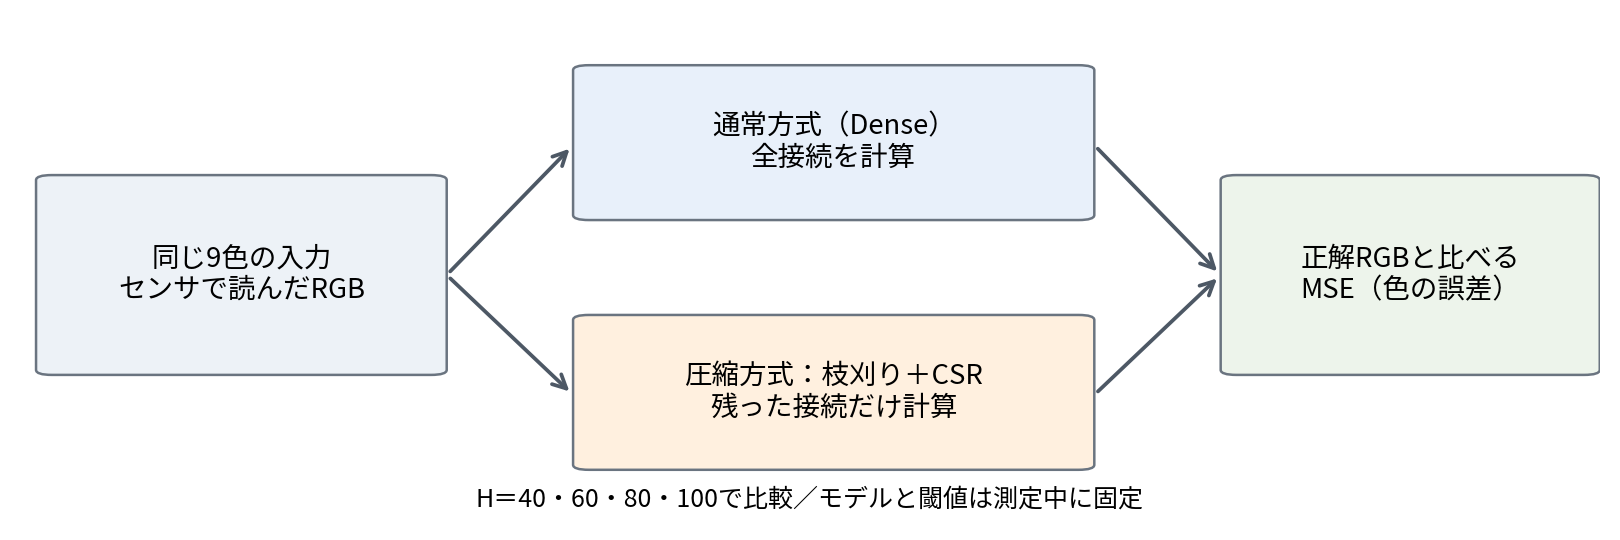
\includegraphics[width=1\textwidth,height=\textheight]{../figures/comparison_flow.png}

\begin{center}同じ入力で比較する流れ\end{center}

\newpage

\section{4　何を使って色を読んだか}\label{ux4f55ux3092ux4f7fux3063ux3066ux8272ux3092ux8aadux3093ux3060ux304b}

\textbf{対応：レポート3.1，図5}

\textbf{「赤・緑・青の光を順番に当て，紙からの反射を光センサで読みました．」}

使用ボードはArduino UNO R4 WiFiで，主マイコンはRA4M1，クロックは48
MHzである．保存用のフラッシュメモリ（Flash）は262,144 byte，RAM（Random
Access Memory）は32,768 byteである．

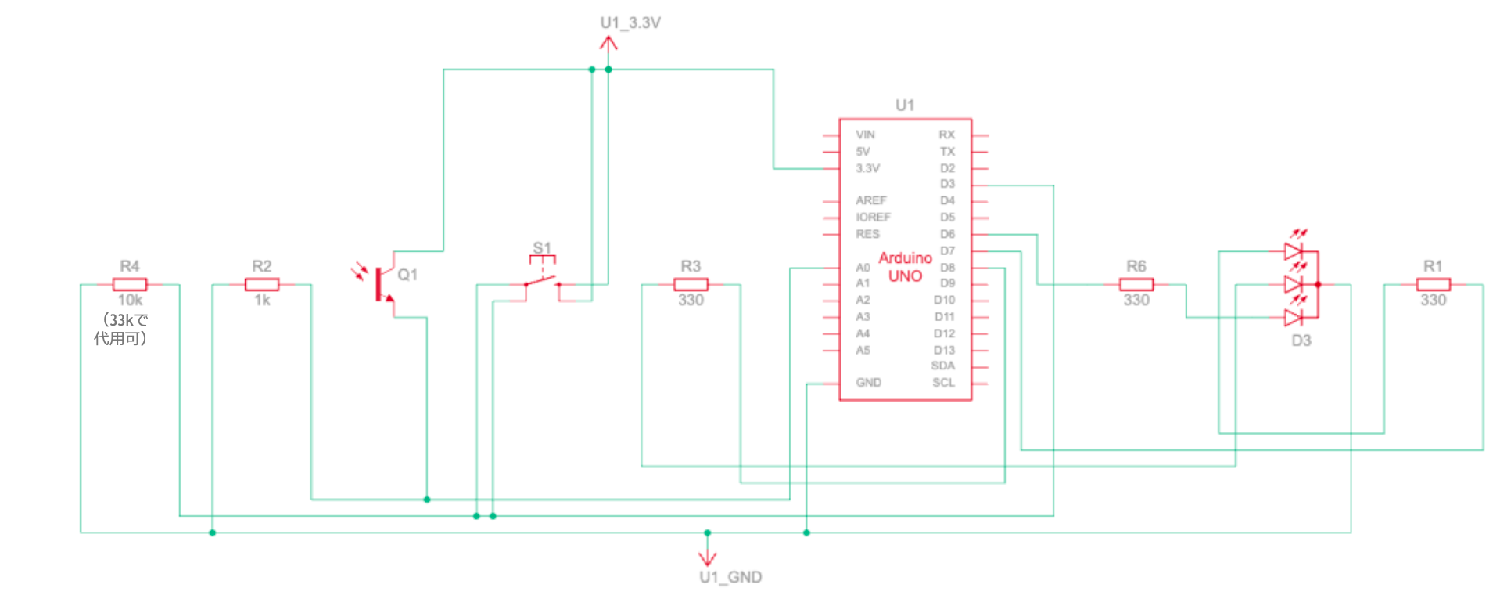
\includegraphics[width=1\textwidth,height=\textheight]{../figures/circuit.pdf}

\begin{center}回路図\end{center}

使用コードでは，赤・緑・青（Red，Green，Blue：RGB）の発光ダイオード（Light
Emitting
Diode：LED）をD8・D6・D7で制御し，受光電圧をA0で読む．LED側の抵抗は各330
Ω，センサ側は1 kΩである．光センサの型番は未確認である．

各色の点灯後10 ms待ち，10サンプルを2
ms間隔で読んで平均した．\texttt{readRGB()}が点灯順を制御し，\texttt{readAverage()}が平均を求める．

\newpage

\section{5　実際の測定手順と保存入力}\label{ux5b9fux969bux306eux6e2cux5b9aux624bux9806ux3068ux4fddux5b58ux5165ux529b}

\textbf{対応：レポート3.5・3.6}

\textbf{「各回で黒白校正を行い，9色を読み終えた時点を1回としました．」}

黒を当ててb，白を当ててwを送り，入力の基準を登録した．その後，赤・緑・青・黄・水色・紫・黒・灰・白の順に紙を当て直し，rを各1回送った．9色の終了後，nで次の回へ進んだ．操作はシリアル通信で行い，外付けボタンは使用していない．

\textbf{1色を読んだ時点で，その入力を全8条件へ渡した．}
DenseとCSRで紙を別々に読み直すと，入力変動と方式差が混ざるためである．重みと閾値は10回の前に固定した．

生の値，黒白校正値，正規化した入力，8条件の出力画像とMSEを保存した．紙は手で支え，距離・角度・照度の数値記録は取っていない．

\textbf{保存入力の実機再生}は，以前に測った入力をArduinoのモデルへ再び与える操作である．紙を新しく読む測定ではない．同じ入力を反復できるため，速度比較に使った．

口頭では「精度は新規10回，速度は保存入力の反復再生です」と分けて説明する．

\newpage

\section{6　学習データと正解は何か}\label{ux5b66ux7fd2ux30c7ux30fcux30bfux3068ux6b63ux89e3ux306fux4f55ux304b}

\textbf{対応：レポート3.2・3.7，付録}

\textbf{「入力はセンサの実測値，正解はその色に対応するRGBです．」}

最終学習には135行を使った．内訳は3×3チャート111行と6×4チャート24行で，同じ色の繰り返しも含む．135種類の異なる色を測った意味ではない．

3×3の教師値と評価には先生指定の\texttt{result.ppm}を使用した．灰色の正解は(127,127,127)である．6×4の24行は，配布Notebookの教師値を使用した．


\includegraphics[width=33mm,height=\textheight]{../color_images/reference.png}

\begin{center}result.ppmの9色\end{center}

学習用の入力で重みを更新し，検証用の入力で枝刈りの閾値を選んだ．新規10回の入力は，その学習・閾値選択に加えていない．

ただし，新規測定も学習と同じ9色の紙である．\textbf{新しく読み直す能力は調べたが，未知の色に対する性能までは確認していない．}

\newpage

\section{7　黒白正規化の式を読む}\label{ux9ed2ux767dux6b63ux898fux5316ux306eux5f0fux3092ux8aadux3080}

\textbf{対応：レポート式(1)，normalizeInput()}

\textbf{「黒を0，白を1とする共通の尺度へ直しました．」}

\[x_c=\operatorname{clip}_{[0,1]}
\left(\frac{v_c-v_{B,c}}{v_{W,c}-v_{B,c}}\right)\]

\(c\)はRGBのいずれか，\(v_c\)は生の読取値，\(v_{B,c}\)は黒，\(v_{W,c}\)は白の校正値である．分子で黒の分を引き，分母で黒から白までの幅を割る．

第1回の赤成分では，実測値から，

\[\frac{137.5-9.8}{186.4-9.8}\approx0.7231\]

となった．コードの中心部分は次である．

\begin{Shaded}
\begin{Highlighting}[]
\DataTypeTok{float}\NormalTok{ range }\OperatorTok{=}\NormalTok{ whiteValue }\OperatorTok{{-}}\NormalTok{ blackValue}\OperatorTok{;}
\DataTypeTok{float}\NormalTok{ result }\OperatorTok{=}
  \OperatorTok{(}\NormalTok{value }\OperatorTok{{-}}\NormalTok{ blackValue}\OperatorTok{)} \OperatorTok{/}\NormalTok{ range}\OperatorTok{;}
\end{Highlighting}
\end{Shaded}

\texttt{range}が0以下なら0を返し，最後に0未満を0，1を超えた値を1へ収める．これがクリップである．異なる生の値でも同じ0へクリップされると，その差はモデルの入力から失われる．

\newpage

\section{8　重み・バイアス・ReLUとは}\label{ux91cdux307fux30d0ux30a4ux30a2ux30b9reluux3068ux306f}

\textbf{対応：レポート式(2)・(4)，図2}

\textbf{「入力を重みで調整して足し，バイアスで全体をずらします．」}

\[z=w_Rx_R+w_Gx_G+w_Bx_B+b\]

重み \(w\) は，入力を何倍して使うかを決める係数である．バイアス \(b\)
は，その合計へ加える調整値である．これらを学習で更新する．

説明用に入力(0.7,0.2,0.1)，重み(0.5,−0.2,0.3)，バイアス0.01なら，

\[z=0.35-0.04+0.03+0.01=0.35\]

となる．負の重みは入力の影響を差し引く．

隠れ層ではRectified Linear Unit（ReLU）を適用する．

\[\operatorname{ReLU}(z)=\max(0,z)\]

0.35はそのまま，−0.2は0になる．この非線形処理を挟むことで，線形変換だけでは表せない関係を学習できる．出力層ではReLUを使わず，RGB変換の直前に0〜1へクリップする．

\newpage

\section{9　3−H−H−3とDenseのコード}\label{hh3ux3068denseux306eux30b3ux30fcux30c9}

\textbf{対応：レポート式(3)，図2}

\textbf{「RGBの3入力から，H個の隠れ層を2回通り，RGBの3出力を得ます．」}

\[\begin{aligned}
\boldsymbol h_1&=\operatorname{ReLU}(W_1\boldsymbol x+\boldsymbol b_1),\\
\boldsymbol h_2&=\operatorname{ReLU}(W_2\boldsymbol h_1+\boldsymbol b_2),\\
\boldsymbol y&=W_3\boldsymbol h_2+\boldsymbol b_3
\end{aligned}\]

重み行列の大きさは順にH×3，H×H，3×Hである．H60はRGBが60成分になる意味ではなく，\textbf{各隠れ層に計算単位が60個ある}という意味である．

Denseの最初の層では，次のように計算する．

\begin{Shaded}
\begin{Highlighting}[]
\DataTypeTok{float}\NormalTok{ value}\OperatorTok{=}\NormalTok{m}\OperatorTok{.}\NormalTok{b1}\OperatorTok{[}\NormalTok{r}\OperatorTok{];}
\ControlFlowTok{for}\OperatorTok{(}\DataTypeTok{int}\NormalTok{ c}\OperatorTok{=}\DecValTok{0}\OperatorTok{;}\NormalTok{c}\OperatorTok{\textless{}}\DecValTok{3}\OperatorTok{;}\NormalTok{c}\OperatorTok{++)}\NormalTok{ value}\OperatorTok{+=}\NormalTok{m}\OperatorTok{.}\NormalTok{w1}\OperatorTok{[}\NormalTok{r}\OperatorTok{*}\DecValTok{3}\OperatorTok{+}\NormalTok{c}\OperatorTok{]*}\NormalTok{input}\OperatorTok{[}\NormalTok{c}\OperatorTok{];}
\NormalTok{layer1}\OperatorTok{[}\NormalTok{r}\OperatorTok{]=}\NormalTok{value}\OperatorTok{\textgreater{}}\FloatTok{0.0}\BuiltInTok{f}\OperatorTok{?}\NormalTok{value}\OperatorTok{:}\FloatTok{0.0}\BuiltInTok{f}\OperatorTok{;}
\end{Highlighting}
\end{Shaded}

\texttt{r}は出力先の単位，\texttt{c}はRGBの成分番号．\texttt{r*3+c}は重み行列を1本の配列へ並べた位置である．\texttt{+=}で積を加算し，最後の条件式でReLUを行う．

両方式とも32ビット単精度浮動小数点形式（32-bit Floating
Point：FP32）で，値1個は4 byteである．整数への量子化は行っていない．

\newpage

\section{10　どうやって重みを学習したか}\label{ux3069ux3046ux3084ux3063ux3066ux91cdux307fux3092ux5b66ux7fd2ux3057ux305fux304b}

\textbf{対応：レポート2.1・3.2，図3}

\textbf{「正解との違いを損失にし，それが減る方向へ重みとバイアスを更新しました．」}

学習はPC（Personal
Computer）側で行い，Arduinoでは学習済みの数値を使って推論した．各Hは同じHのV9重みを読み込み，40,000回追加更新した．乱数シードは42である．

\begin{Shaded}
\begin{Highlighting}[]
\NormalTok{optimizer.zero\_grad()}\OperatorTok{;}\NormalTok{ prediction}\OperatorTok{=}\NormalTok{model(ax)}
\CommentTok{\# この間に次ページの損失を計算する}
\ControlFlowTok{assert}\NormalTok{ torch.isfinite(loss)}
\NormalTok{loss.backward()}\OperatorTok{;}\NormalTok{ optimizer.step()}\OperatorTok{;}\NormalTok{ schedule.step()}
\end{Highlighting}
\end{Shaded}

\texttt{zero\_grad()}は前回の勾配を消し，\texttt{model(ax)}は入力から予測を求める．その後，次ページの式で\texttt{loss}を求める．

\texttt{backward()}は，各重みを少し変えると損失がどちらへ変わるかを計算する．この情報が勾配である．\texttt{step()}はAdam（Adaptive
Moment Estimation）で実際の数値を更新する．

学習率は更新の大きさを調整する．コサイン状に0.0005から0.000005へ下げた．最初は比較的大きく動かし，後半は小さく調整する設定である．

\textbf{40,000回は最終V10の追加更新回数であり，モデルの全履歴を最初から学習した総回数ではない．}

\newpage

\section{11　学習損失の式全体を読む}\label{ux5b66ux7fd2ux640dux5931ux306eux5f0fux5168ux4f53ux3092ux8aadux3080}

\textbf{対応：レポート式(5)}

\textbf{「色の間違いの点数と，大きな重みへの罰則を足した式です．」}

\[E_i=\frac13\sum_{c\in\{R,G,B\}}
\rho_\beta(\widehat y_{i,c}-t_{i,c})\]

\[\mathcal L=
\frac{\sum_{i=1}^{M}a_iE_i}{\sum_{i=1}^{M}a_i}
+10^{-6}\sum_{\ell=1}^{3}\sum_{j,k}|(W_\ell)_{jk}|\]

\(M=135\)は学習行数，\(\widehat y\)は予測，\(t\)は正解である．RGBの3成分を平均して1行分の点数
\(E_i\) を作る．学習時のRGB尺度は0〜1である．

前半は，重要度を掛けた点数の合計を，重要度の合計で割る．前に「1／重要度の合計」を掛ける書き方と同じで，1は割り算のための係数，\(a_i\)は各行の点数へ掛ける係数である．

後半は3層の重みの絶対値を足したL1正則化である．バイアスは対象に含めない．例えば重みが0.1，−0.2，0なら，絶対値の合計は0.3となる．

\textbf{行の重要度 \(a_i\) と，ネットワークの接続の重み \(W\)
は別物である．}
L1は小さい重みを作る方向に作用し，実際に0へするのは後の枝刈りである．

\newpage

\section{12　Smooth
L1を使った理由}\label{smooth-l1ux3092ux4f7fux3063ux305fux7406ux7531}

\textbf{対応：レポート式(6)，学習コード}

\textbf{「大きな残差に引っ張られすぎないよう，誤差の点数の増え方を変えました．」}

\[\rho_\beta(e)=
\begin{cases}
e^2/(2\beta)&(|e|<\beta),\\
|e|-\beta/2&(|e|\geq\beta)
\end{cases}
\qquad\beta=0.05\]

\(e\)は予測−正解である．条件に合う片方だけを使う．小さい誤差は二乗，大きい誤差は直線的に損失を増やす．

説明用に，\(e=0.02\)なら \(0.02^2/0.1=0.004\)，\(e=0.1\)なら
\(0.1-0.025=0.075\) となる．

\begin{Shaded}
\begin{Highlighting}[]
\NormalTok{loss\_rows }\OperatorTok{=}\NormalTok{ F.smooth\_l1\_loss(}
\NormalTok{    prediction, ty,}
\NormalTok{    beta}\OperatorTok{=}\FloatTok{.05}\NormalTok{, reduction}\OperatorTok{=}\StringTok{\textquotesingle{}none\textquotesingle{}}
\NormalTok{).mean(}\DecValTok{1}\NormalTok{)}
\end{Highlighting}
\end{Shaded}

\texttt{reduction=\textquotesingle{}none\textquotesingle{}}で成分別に残し，\texttt{.mean(1)}でRGBを平均する．次に行重要度とL1項を使う．

\begin{Shaded}
\begin{Highlighting}[]
\NormalTok{loss}\OperatorTok{=}\NormalTok{(loss\_rows}\OperatorTok{*}\NormalTok{weights).}\BuiltInTok{sum}\NormalTok{()}\OperatorTok{/}\NormalTok{weights.}\BuiltInTok{sum}\NormalTok{()}\OperatorTok{+}\FloatTok{1e{-}6}\OperatorTok{*}\BuiltInTok{sum}\NormalTok{(p.}\BuiltInTok{abs}\NormalTok{().}\BuiltInTok{sum}\NormalTok{() }\ControlFlowTok{for}\NormalTok{ name,p }\KeywordTok{in}\NormalTok{ model.named\_parameters() }\ControlFlowTok{if} \StringTok{\textquotesingle{}weight\textquotesingle{}} \KeywordTok{in}\NormalTok{ name)}
\end{Highlighting}
\end{Shaded}

\texttt{weights}は行重要度，\texttt{p}は学習パラメータである．名前に\texttt{weight}を含むものだけをL1項へ足し，バイアスを除く．

\textbf{Smooth L1は学習の点数，MSEは評価の指標である．}
損失の減少と，MSE300以下は同じ条件ではない．

\newpage

\section{13　重要度とデータ拡張の意味}\label{ux91cdux8981ux5ea6ux3068ux30c7ux30fcux30bfux62e1ux5f35ux306eux610fux5473}

\textbf{対応：レポート3.2・3.7，data\_weights.py}

\textbf{「同じ色の重複数を調整し，読取値の変動も学習に加えました．」}

3×3の行重要度は，色ごとの寄与をそろえ，さらに校正グループと同一グループ内の重複数で分けた．一部の行数が多いだけで，その色が極端に強く影響するのを避ける設定である．

古い読取群には，近い入力5件の教師値との整合度も反映した．整合度の係数には下限0.1を置き，全135行を正の重要度で残した．詳細な値は学習重要度CSVに保存した．

説明用に，行の点数2と4，重要度1と3なら，

\[\frac{1\times2+3\times4}{1+3}=3.5\]

となる．

データ拡張では，3×3入力の50\%にRGB別のgain
0.75〜1.30とoffsetを加えた．灰・白は30\%の確率で共通gain
0.5〜1.15も適用した．offset幅は，異なる教師値をもつ学習入力間の距離から決めた．

gainは掛け算，offsetは足し算の調整である．\textbf{学習中の変換なので，物理測定の回数は増えない．}
新規10回の入力は拡張や重要度の計算にも使用していない．

\newpage

\section{14　何を枝刈りしたか}\label{ux4f55ux3092ux679dux5208ux308aux3057ux305fux304b}

\textbf{対応：レポート式(7)，図4}

\textbf{「学習後に，絶対値が閾値より小さい接続の重みを0にしました．」}

\[w^{(\tau)}=
\begin{cases}
0&(|w|<\tau),\\
w&(|w|\geq\tau)
\end{cases}\]

\(\tau\)はどこまで削るかを決める閾値である．正負ではなく絶対値で判定する．バイアスは削らない．

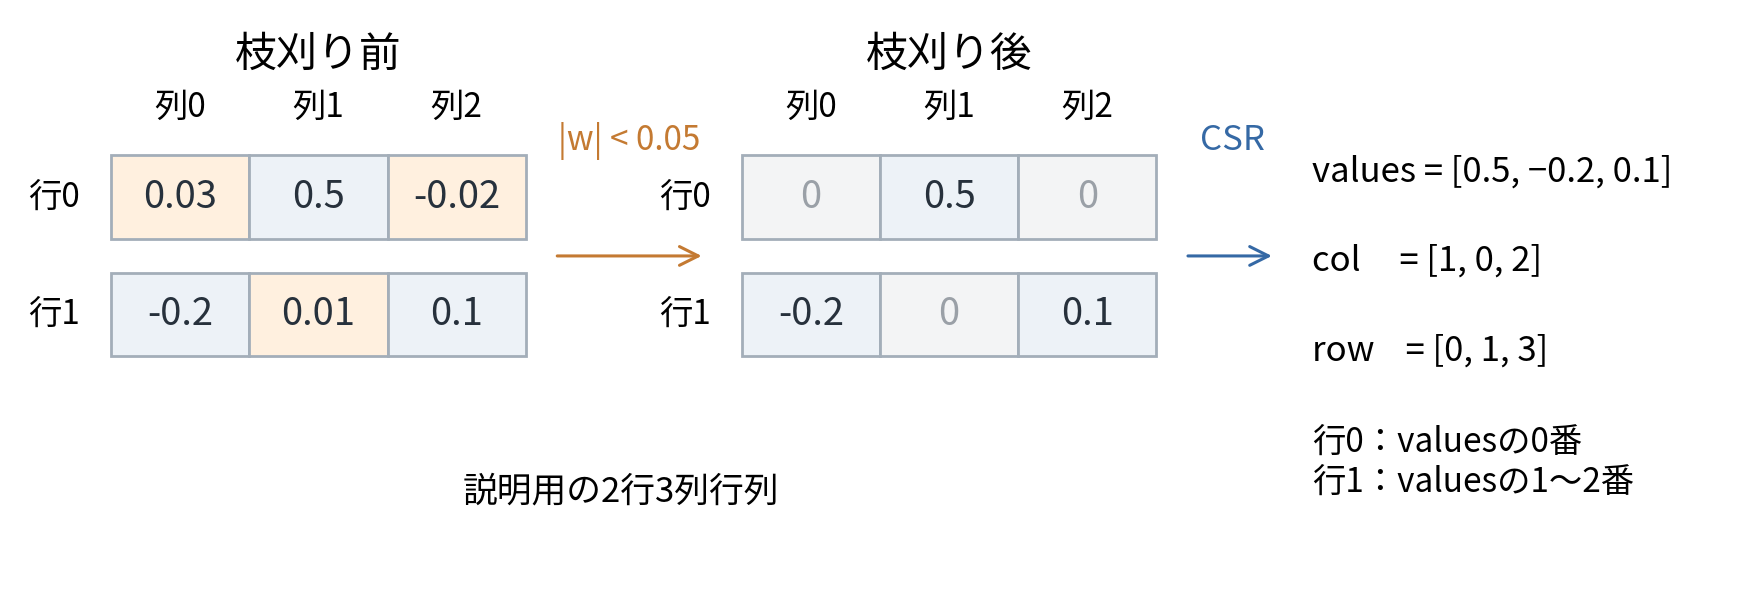
\includegraphics[width=1\textwidth,height=\textheight]{../figures/theory_pruning_csr.png}

\begin{center}枝刈りとCSRの説明例\end{center}

H60の採用閾値は約0.05434179である．説明用に0.03，−0.02は0となり，0.2は残る．重みを削ると，途中の計算値やReLUの結果も変わり，最終的なRGBへ影響する．

閾値を大きくするほど一般に多くの重みを削れるが，精度も変わる．\textbf{このV10では，枝刈り後の再学習は行っていない．}
再学習は今後の改善案である．

Smooth L1の \(\beta\) は損失の切替値，枝刈りの \(\tau\)
は削除判定値であり，用途が異なる．

\newpage

\section{15　閾値は何を基準に選んだか}\label{ux95beux5024ux306fux4f55ux3092ux57faux6e96ux306bux9078ux3093ux3060ux304b}

\textbf{対応：レポート3.4の表}

\textbf{「新規10回を始める前に，検証入力で条件を満たす最小容量の候補を選びました．」}

候補は学習済み重みの絶対値を並べ，隣接する異なる値の中間から作った．候補数は固定していない．次の3条件を満たす候補から選んだ．

\begin{enumerate}
\def\labelenumi{\arabic{enumi}.}
\tightlist
\item
  検証128入力でDenseに対するMSE増加5\%以下
\item
  CSR配列容量がDenseより小さい
\item
  学習内V8の9入力でMSE300以下
\end{enumerate}

\begin{longtable}[]{@{}lrr@{}}
\toprule\noalign{}
H & 検証Dense & 検証CSR \\
\midrule\noalign{}
\endhead
\bottomrule\noalign{}
\endlastfoot
40 & 5012.20 & 4715.84 \\
60 & 5226.80 & 5292.58 \\
80 & 5135.43 & 4553.44 \\
100 & 5237.21 & 4632.38 \\
\end{longtable}

\textbf{この表は最終の新規10回とは入力が違う．}
8×8の別チャートなので，MSEが約5,000でも新規9色の平均値とは矛盾しない．

検証2回目は異なる6色が同じ(0,0,0)入力になっていた．同じ入力から異なる色を出し分けることはできず，選択の信頼性には制約がある．検証1回目も誤差が大きく，入力衝突だけが原因とは断定できない．選択は暫定として扱った．

\newpage

\section{16　CSRの3配列を例で説明する}\label{csrux306e3ux914dux5217ux3092ux4f8bux3067ux8aacux660eux3059ux308b}

\textbf{対応：レポート2.2，図4}

\textbf{「残った値と列番号を並べ，rowで行の区切りを示します．」}

以下は説明用の2行3列の行列である．番号は0から数える．

\begin{Shaded}
\begin{Highlighting}[]
\NormalTok{        列0   列1  列2}
\NormalTok{行0      0    0.5   0}
\NormalTok{行1    {-}0.2    0   0.1}

\NormalTok{values = [0.5, {-}0.2, 0.1]}
\NormalTok{col    = [1,    0,   2  ]}
\NormalTok{row    = [0,    1,   3  ]}
\end{Highlighting}
\end{Shaded}

\texttt{values{[}k{]}}が重み，\texttt{col{[}k{]}}が元の列番号である．行rでは\texttt{row{[}r{]}}から\texttt{row{[}r+1{]}}の手前までを読む．

行0はk＝0だけ，行1はk＝1，2を使う．最後の3は終端であり，\texttt{values{[}3{]}}を読む指定ではない．rowの個数は行数＋1になる．

入力(1,2,3)，バイアス0なら，行0は \(0.5\times2=1\)，行1は
\(-0.2\times1+0.1\times3=0.1\) となる．

\textbf{CSRは枝刈り後の行列の表現を変える処理である．}
正しく変換すれば，削った後の通常行列と同じ計算ができる．

\newpage

\section{17　CSR推論コードを説明する}\label{csrux63a8ux8ad6ux30b3ux30fcux30c9ux3092ux8aacux660eux3059ux308b}

\textbf{対応：レポート3.3，付録のコード}

\textbf{「各行について，残った重みだけの積を足します．」}

実際の\texttt{sparseLayer()}の本体を，改行と説明コメントを付けて示す．

\begin{Shaded}
\begin{Highlighting}[]
\CommentTok{// 出力の各行を順番に計算する}
\ControlFlowTok{for} \OperatorTok{(}\DataTypeTok{int}\NormalTok{ r}\OperatorTok{=}\DecValTok{0}\OperatorTok{;}\NormalTok{ r}\OperatorTok{\textless{}}\NormalTok{layer}\OperatorTok{.}\NormalTok{rows}\OperatorTok{;}\NormalTok{ r}\OperatorTok{++)} \OperatorTok{\{}
  \CommentTok{// バイアスから始める}
  \DataTypeTok{float}\NormalTok{ value}\OperatorTok{=}\NormalTok{layer}\OperatorTok{.}\NormalTok{bias}\OperatorTok{[}\NormalTok{r}\OperatorTok{];}
  \CommentTok{// この行の非ゼロ重みだけを使う}
  \ControlFlowTok{for} \OperatorTok{(}\DataTypeTok{uint16\_t}\NormalTok{ k}\OperatorTok{=}\NormalTok{layer}\OperatorTok{.}\NormalTok{row}\OperatorTok{[}\NormalTok{r}\OperatorTok{];}
\NormalTok{       k}\OperatorTok{\textless{}}\NormalTok{layer}\OperatorTok{.}\NormalTok{row}\OperatorTok{[}\NormalTok{r}\OperatorTok{+}\DecValTok{1}\OperatorTok{];}\NormalTok{ k}\OperatorTok{++)}
\NormalTok{    value }\OperatorTok{+=}\NormalTok{ layer}\OperatorTok{.}\NormalTok{values}\OperatorTok{[}\NormalTok{k}\OperatorTok{]}
           \OperatorTok{*}\NormalTok{ input}\OperatorTok{[}\NormalTok{layer}\OperatorTok{.}\NormalTok{col}\OperatorTok{[}\NormalTok{k}\OperatorTok{]];}
  \CommentTok{// 隠れ層だけReLUを使う}
\NormalTok{  output}\OperatorTok{[}\NormalTok{r}\OperatorTok{]=(}\NormalTok{relu }\OperatorTok{\&\&}\NormalTok{ value}\OperatorTok{\textless{}}\DecValTok{0}\OperatorTok{)}
          \OperatorTok{?} \DecValTok{0} \OperatorTok{:}\NormalTok{ value}\OperatorTok{;}
\OperatorTok{\}}
\end{Highlighting}
\end{Shaded}

\texttt{r}は出力の番号，\texttt{k}は圧縮した配列内の番号である．\texttt{col{[}k{]}}で掛ける入力を探すため，\textbf{kと元の列番号は同じとは限らない．}

\texttt{predict()}はこの層計算を3回呼び，隠れ層2つでは\texttt{relu=true}，出力層では\texttt{false}とする．0を掛ける計算は省けるが，位置情報を読む処理は追加される．

\newpage

\section{18　NNZとDenseの容量を計算する}\label{nnzux3068denseux306eux5bb9ux91cfux3092ux8a08ux7b97ux3059ux308b}

\textbf{対応：レポート式(8)・(9)，表3}

\textbf{「接続数とバイアス数を数え，1個4 byteを掛けました．」}

非ゼロ要素数（Number of
Nonzeros：NNZ）は，今回は3層に残った重みの総数Kである．バイアスはNNZに数えない．

元の重み数とバイアス数は，

\[N_w=3H+H^2+3H=H^2+6H\] \[N_b=H+H+3=2H+3\]

なので，FP32のDense配列容量は，

\[B_{\mathrm{Dense}}=4(H^2+8H+3)\]

となる．H60なら重み3,960個，バイアス123個で，\((3,960+123)\times4=16,332\)
byteである．

式(8)の疎性Sは，0になった重みの割合である．

\[S=1-\frac{K}{H^2+6H}\]

H60ではK＝1,141なので，重みの約71.19\%が0となる．この割合は，位置情報やバイアスも含めた配列容量の削減率とは異なる．

\newpage

\section{19　CSRの容量と成立条件を計算する}\label{csrux306eux5bb9ux91cfux3068ux6210ux7acbux6761ux4ef6ux3092ux8a08ux7b97ux3059ux308b}

\textbf{対応：レポート式(10)・(11)・(12)}

\textbf{「値の容量に，列・行の位置情報とバイアスを足します．」}

\[\begin{aligned}
B_{\mathrm{CSR}}
&=4K+K+2(2H+6)+4(2H+3)\\
&=5K+12H+24
\end{aligned}\]

\texttt{values}はFP32で4K byte，\texttt{col}は8ビット整数でK
byte，\texttt{row}は16ビット整数で1個2
byteである．バイアスはFP32のまま全て残す．

行位置の個数は，層ごとに行数＋1なので，\((H+1)+(H+1)+(3+1)=2H+6\)
となる．

H60では，4,564＋1,141＋252＋492＝\textbf{6,449 byte}．Denseの16,332
byteから60.51\%削減した．

小さくなる条件は \(B_{\mathrm{CSR}}<B_{\mathrm{Dense}}\) を整理して，

\[5K<4H^2+20H-12\]

となる．位置情報にも容量が必要なので，ほとんど重みを削れない場合にはCSRが小さくならない．本実装の列番号は8ビット，行位置は16ビットなので，大きなHへ拡張する際は型の上限も確認する．

\newpage

\section{20　出力とMSEをどう計算したか}\label{ux51faux529bux3068mseux3092ux3069ux3046ux8a08ux7b97ux3057ux305fux304b}

\textbf{対応：レポート式(13)，outputTo255()}

\textbf{「出力を整数RGBにし，正解との差を二乗して27成分で平均しました．」}

モデル出力を0〜1へクリップし，255倍して0.5を加え，整数へ変換する．非負値をこの方法で四捨五入する．

\[\mathrm{MSE}=\frac1{27}
\sum_{i=1}^{9}\sum_{c\in\{R,G,B\}}(y_{i,c}-t_{i,c})^2\]

9色×3成分なので27で割る．符号を消すため二乗し，大きく外れた成分ほど強く反映する．小さいほど正解に近く，0なら27成分全てが一致する．

説明用に1色だけが正解(255,0,0)，予測(245,10,5)で，他の8色が一致した場合，MSEは
\((100+100+25)/27=8.33\ldots\) である．

保存入力版の実コードの計算部分を示す．

\begin{Shaded}
\begin{Highlighting}[]
\DataTypeTok{int}\NormalTok{ e}\OperatorTok{=}\KeywordTok{static\_cast}\OperatorTok{\textless{}}\DataTypeTok{int}\OperatorTok{\textgreater{}(}
\NormalTok{  pixels}\OperatorTok{[}\NormalTok{model}\OperatorTok{][}\NormalTok{point}\OperatorTok{][}\NormalTok{c}\OperatorTok{])}
  \OperatorTok{{-}}\NormalTok{trained\_models}\OperatorTok{::}\NormalTok{REFERENCE\_RGB}\OperatorTok{[}\NormalTok{point}\OperatorTok{][}\NormalTok{c}\OperatorTok{];}
\NormalTok{mse}\OperatorTok{[}\NormalTok{model}\OperatorTok{]+=}\KeywordTok{static\_cast}\OperatorTok{\textless{}}\DataTypeTok{double}\OperatorTok{\textgreater{}(}\NormalTok{e}\OperatorTok{)*}\NormalTok{e}\OperatorTok{/}\FloatTok{27.0}\OperatorTok{;}
\end{Highlighting}
\end{Shaded}

RGBへ変換する四捨五入と，MSE表示の小数第3位以降の切り捨ては別の処理である．MSE300は「RGBが300ずれた」意味ではなく，差の二乗の平均である．

\newpage

\section{21　平均と標本SDの意味}\label{ux5e73ux5747ux3068ux6a19ux672csdux306eux610fux5473}

\textbf{対応：レポート式(14)，表1}

\textbf{「平均で誤差の大きさ，SDで読取ごとのばらつきを見ました．」}

各回のMSEを \(m_r\) とすると，

\[\overline m=\frac{m_1+\cdots+m_{10}}{10}\]

である．今回は全回9色なので，各回MSEの平均は，90色270成分の二乗誤差をまとめて平均した値とも一致する．平均した画像からMSEを計算したものではない．

標本標準偏差（Standard Deviation：SD）は，

\[s_m=\sqrt{\frac1{9}
\sum_{r=1}^{10}(m_r-\overline m)^2}\]

である．各回が平均から離れた量を二乗して足し，標本SDの定義に従い10−1＝9で割り，平方根を取る．SDが大きいほど回ごとの違いが大きい．

H60
Denseは平均238.33，標本SD738.23だった．良い回が多くても，1回の大きな誤差が平均とSDへ強く影響する．

このSDは読取10回のばらつきである．速度表の±は100推論×5組のばらつきで，観測単位が異なる．

\newpage

\section{22　方式差と増加率の式を読む}\label{ux65b9ux5f0fux5deeux3068ux5897ux52a0ux7387ux306eux5f0fux3092ux8aadux3080}

\textbf{対応：レポート式(15)・(16)・(17)，表2}

\textbf{「同じ回の差と，10回平均の比を使って比較しました．」}

\[d_r=m_{r,\mathrm{CSR}}-m_{r,\mathrm{Dense}}\]

正ならCSRの誤差が増え，負なら減ったことを示す．同じ入力同士で引くため，方式による違いを比較できる．

平均MSEの増加率は，

\[R_{\mathrm{MSE}}=
100\left(\frac{\overline m_{\mathrm{CSR}}}
{\overline m_{\mathrm{Dense}}}-1\right)\]

である．H60では238.33→493.51，増加率は107.06\%となる．各回の増加率10個を平均した値ではない．

容量と時間は，減った割合を求めるので，

\[\begin{aligned}
R_B&=100\left(1-\frac{B_{\mathrm{CSR}}}{B_{\mathrm{Dense}}}\right),\\
R_T&=100\left(1-\frac{T_{\mathrm{CSR}}}{T_{\mathrm{Dense}}}\right)
\end{aligned}\]

とする．MSE増加率は正なら悪化，削減率は正なら改善を示す．切り捨て前の値から計算した．

\newpage

\section{23　精度の結果を数字で説明する}\label{ux7cbeux5ea6ux306eux7d50ux679cux3092ux6570ux5b57ux3067ux8aacux660eux3059ux308b}

\textbf{対応：レポート4.1，表1・2}

\textbf{「Denseは3条件で平均300以下でしたが，CSRは全条件で平均300を超えました．」}

\begin{longtable}[]{@{}lrr@{}}
\toprule\noalign{}
H & Dense平均MSE & CSR平均MSE \\
\midrule\noalign{}
\endhead
\bottomrule\noalign{}
\endlastfoot
40 & 319.56 & 452.04 \\
60 & 238.33 & 493.51 \\
80 & 231.68 & 465.72 \\
100 & 260.42 & 651.92 \\
\end{longtable}

\begin{longtable}[]{@{}lrr@{}}
\toprule\noalign{}
H & Denseの300以下 & CSRの300以下 \\
\midrule\noalign{}
\endhead
\bottomrule\noalign{}
\endlastfoot
40 & 9/10 & 9/10 \\
60 & 9/10 & 9/10 \\
80 & 9/10 & 8/10 \\
100 & 8/10 & 0/10 \\
\end{longtable}

Denseの平均が最小だったのはH80である．ただし，Hを大きくすれば単調に改善したわけではない．

全H・全10回で，CSRのMSEが同じ回のDenseを上回った．平均MSEの増加率は41.46〜150.33\%で，\textbf{精度維持の条件「増加5\%以下」は達成しなかった．}

「300以下の回が9回ある」と「10回平均が300以下」は別である．H40では9回が300以下でも，高誤差の回を含む平均は319.56となった．

\newpage

\section{24　第2回と画像・グラフの読み方}\label{ux7b2c2ux56deux3068ux753bux50cfux30b0ux30e9ux30d5ux306eux8aadux307fux65b9}

\textbf{対応：レポート4.1・5.1，図6，付録}

\textbf{「第2回は全条件で誤差が大きく，操作ミスの申告がなかったため，そのまま集計しました．」}

\begin{center}
\begin{tabular}{cc}

\includegraphics[width=37mm]{../color_images/capture_01/h60_dense.png}&

\includegraphics[width=37mm]{../color_images/capture_02/h60_dense.png}\\
第1回のH60 Dense&第2回のH60 Dense
\end{tabular}
\end{center}

第1回のMSEは2.66，第2回は2339.37である．同じモデルでも，入力が変わると色が大きく変わることが分かる．この10回平均が238.33である．

青・水色のRAWや正規化入力も他の回と異なっていた．校正・紙の位置・照射・センサ応答が原因候補だが，原因を分離して測っていないため，特定はできない．

図6の横軸は読取回，縦軸はMSEの対数目盛である．同じ縦幅は同じ差ではなく同じ倍率を表す．破線は300，線で結んでいても連続時間の変化ではなく各回の結果である．

\textbf{画像1枚のMSEはその回の値であり，10回平均を代表する画像ではない．}

\newpage

\section{25　配列容量はどれだけ減ったか}\label{ux914dux5217ux5bb9ux91cfux306fux3069ux308cux3060ux3051ux6e1bux3063ux305fux304b}

\textbf{対応：レポート4.2，表3，図7の容量側}

\textbf{「索引とバイアスも含めて，モデル配列が約61〜70\%小さくなりました．」}

\begin{longtable}[]{@{}lrr@{}}
\toprule\noalign{}
H & Dense byte & CSR byte \\
\midrule\noalign{}
\endhead
\bottomrule\noalign{}
\endlastfoot
40 & 7,692 & 2,854 \\
60 & 16,332 & 6,449 \\
80 & 28,172 & 9,229 \\
100 & 43,212 & 13,094 \\
\end{longtable}

H60では16,332→6,449
byteで60.51\%削減した．残した重みは3,960個中1,141個である．位置情報の分も含めて小さくなっている．

最小容量はH40 CSRの2,854
byteである．最大削減率はH100の69.70\%である．\textbf{最も小さいモデルと，削減率が最大のモデルは同じではない．}

ここで数えているのは，重み・バイアス・CSR索引の数値配列だけである．プログラムの命令やArduinoの共通処理は含まない．それらを含むFlash全体は28で別に説明する．

Denseは \(H^2\)
の項をもつので，Hが増えると保存量が大きくなりやすい．CSRは残った重み数Kに依存するため，Hだけで容量を決めることはできない．

\newpage

\section{26　速度計測コードを説明する}\label{ux901fux5ea6ux8a08ux6e2cux30b3ux30fcux30c9ux3092ux8aacux660eux3059ux308b}

\textbf{対応：レポート3.6，付録のコード}

\textbf{「100回分の経過時間を測り，100で割って1推論の時間にしました．」}

\texttt{timeModel()}の計時部分を，改行とコメントを付けて示す．

\begin{Shaded}
\begin{Highlighting}[]
\DataTypeTok{float}\NormalTok{ output}\OperatorTok{[}\DecValTok{3}\OperatorTok{];}\NormalTok{ checksum}\OperatorTok{=}\DecValTok{0}\OperatorTok{;}
\CommentTok{// 開始時刻}
\DataTypeTok{uint32\_t}\NormalTok{ begin}\OperatorTok{=}\KeywordTok{static\_cast}\OperatorTok{\textless{}}\DataTypeTok{uint32\_t}\OperatorTok{\textgreater{}(}\NormalTok{micros}\OperatorTok{());}
\ControlFlowTok{for} \OperatorTok{(}\DataTypeTok{int}\NormalTok{ call}\OperatorTok{=}\DecValTok{0}\OperatorTok{;}\NormalTok{ call}\OperatorTok{\textless{}}\DecValTok{100}\OperatorTok{;}\NormalTok{ call}\OperatorTok{++)} \OperatorTok{\{}
  \CommentTok{// 保存済み9入力から選ぶ}
  \DataTypeTok{int}\NormalTok{ input}\OperatorTok{=(}\NormalTok{group}\OperatorTok{*}\DecValTok{100}\OperatorTok{+}\NormalTok{call}\OperatorTok{)}
    \OperatorTok{\%}\NormalTok{ comparison\_models}\OperatorTok{::}\NormalTok{BENCHMARK\_INPUT\_COUNT}\OperatorTok{;}
\NormalTok{  comparison\_models}\OperatorTok{::}\NormalTok{predict}\OperatorTok{(}
\NormalTok{    model}\OperatorTok{,}
\NormalTok{    comparison\_models}\OperatorTok{::}\NormalTok{BENCHMARK\_INPUTS}\OperatorTok{[}\NormalTok{input}\OperatorTok{],}
\NormalTok{    output}\OperatorTok{);}
  \CommentTok{// 出力を使用する}
\NormalTok{  checksum}\OperatorTok{+=}\NormalTok{output}\OperatorTok{[}\DecValTok{0}\OperatorTok{]+}\NormalTok{output}\OperatorTok{[}\DecValTok{1}\OperatorTok{]+}\NormalTok{output}\OperatorTok{[}\DecValTok{2}\OperatorTok{];}
\OperatorTok{\}}
\CommentTok{// 終了時刻との差}
\ControlFlowTok{return} \KeywordTok{static\_cast}\OperatorTok{\textless{}}\DataTypeTok{uint32\_t}\OperatorTok{\textgreater{}(}\NormalTok{micros}\OperatorTok{()){-}}\NormalTok{begin}\OperatorTok{;}
\end{Highlighting}
\end{Shaded}

\texttt{micros()}はマイクロ秒単位の時刻を返す．\texttt{\%}は余りで，保存した9入力を巡回する．\texttt{checksum}へ出力を足し，計算結果を実際に利用している．

計時には入力選択・推論・出力合計を含む．センサ読取・シリアル表示・MSE計算は含めない．このコードが返すのは100回の合計時間である．

\newpage

\section{27　速度の結果と短縮の理由}\label{ux901fux5ea6ux306eux7d50ux679cux3068ux77edux7e2eux306eux7406ux7531}

\textbf{対応：レポート4.3・5.1，表4，図7}

\textbf{「全Hで速くなりましたが，掛け算が減った割合ほど時間は減りませんでした．」}

\begin{longtable}[]{@{}lrrr@{}}
\toprule\noalign{}
H & Dense µs & CSR µs & 短縮率 \\
\midrule\noalign{}
\endhead
\bottomrule\noalign{}
\endlastfoot
40 & 465.262 & 305.834 & 34.27\% \\
60 & 945.648 & 671.674 & 28.97\% \\
80 & 1593.368 & 956.212 & 39.99\% \\
100 & 2408.160 & 1348.392 & 44.01\% \\
\end{longtable}

H60は945.648→671.674
µsで28.97\%短縮した．H100は44.01\%短縮したが，最短の絶対時間はH40
CSRの305.834 µsである．

H60では，重みと入力を掛ける回数が3,960→1,141回となり71.19\%減った．ただし，CSRでは列・行の位置情報を読み，ループを制御する処理も必要になる．そのため，掛け算の削減率と時間短縮率は一致しない．各処理の内訳時間は測っていない．

最初に各条件10推論をウォームアップし，100推論×5組の平均を求めた．Dense先行とCSR先行を交互にし，順番が一方へ偏らないようにした．

図7の時間側の誤差棒は，\textbf{5組の平均時間の標本SD}であり，500推論それぞれのSDではない．紙を移動する時間も含まない．

\newpage

\section{28　FlashとRAMはどうなったか}\label{flashux3068ramux306fux3069ux3046ux306aux3063ux305fux304b}

\textbf{対応：レポート4.4，表5・6，図8}

\textbf{「単独モデルのFlashは減りましたが，静的RAMは全8条件で同じでした．」}

\begin{longtable}[]{@{}lrr@{}}
\toprule\noalign{}
H & Dense Flash & CSR Flash \\
\midrule\noalign{}
\endhead
\bottomrule\noalign{}
\endlastfoot
40 & 60,852 & 56,020 \\
60 & 69,492 & 59,612 \\
80 & 81,348 & 62,396 \\
100 & 96,388 & 66,260 \\
\end{longtable}

単位はbyte．H60は14.22\%，H100は31.26\%減少した．Arduinoの共通処理も残るので，モデル配列だけの削減率より小さい．

単独比較の静的RAMは全8条件で\textbf{6,764
byte}，静的割当後の残りは26,004
byteだった．\texttt{const}のモデル配列容量と，静的RAM表示は同じものではない．正確な配置を調べるリンカマップは保存していない．

中間計算には\texttt{float{[}100{]}}を2本使い，宣言上は800
byteである．関数内のこの配列は静的RAM表示に含まれない．\textbf{最大スタック量は未測定なので，残り26,004
byteを実際に使ったとは言えない．}

全8条件入りの新規読取版はFlash191,320／静的RAM7,324
byte，速度版は187,888／6,740
byteだった．単独モデル版とは機能と搭載数が異なる．

\newpage

\section{29　コードと計算の確認方法}\label{ux30b3ux30fcux30c9ux3068ux8a08ux7b97ux306eux78baux8a8dux65b9ux6cd5}

\textbf{対応：レポート3.3・4.4，付録}

\textbf{「索引・固定入力・実測出力・MSEを，それぞれ照合しました．」}

\texttt{validIndices()}はrowの開始・終端・単調性，colの範囲と順序を調べる．\texttt{selfCheckAll()}は固定12入力に対する全8条件の出力を，PCで作った参照値と比較する．

\textbf{CSRの正しさは，枝刈り後の通常行列と比べる．}
元のDenseとの出力差は，重みを削った影響も含むため，それだけでCSR変換の不具合とは判定しない．

新規10回の全80PPM，計2,160成分は，保存した入力を固定V10へ通したPC再計算と一致した．MSE80個は先生の計算サイトの方法とも表示桁の範囲で一致した．これは実装・集計の一致であり，精度が高いという意味ではない．

\textbf{使ったファイルの流れ}

PC側の学習・変換・集計に使った主なファイルを示す．Arduinoでは\texttt{predict()}で推論する．

\begin{Shaded}
\begin{Highlighting}[]
\NormalTok{train.py                      学習}
\NormalTok{select\_compression.py         閾値候補の比較}
\NormalTok{finalize\_compression.py       閾値の固定}
\NormalTok{build\_program.py              数値ヘッダへ出力}
\NormalTok{record\_fresh\_capture.py       読取ログの検算}
\NormalTok{record\_single\_model\_memory.py 単独表示の記録}
\end{Highlighting}
\end{Shaded}

\newpage

\section{30　おわりにをどう説明するか}\label{ux304aux308fux308aux306bux3092ux3069ux3046ux8aacux660eux3059ux308bux304b}

\textbf{対応：レポート3.7・5章}

\textbf{「容量と速度の改善は確認しましたが，精度維持との両立はできませんでした．」}

モデル配列は60.51〜69.70\%，推論時間は28.97〜44.01\%，単独Flashは7.94〜31.26\%減った．静的RAMは変わらなかった．一方，CSRの平均MSE300以下と，Denseからの増加5\%以下は全Hで達成しなかった．

当初から変えた点は，学習データを33組から135行へ増やしたこと，入力変動へ対応するデータ拡張と重み付きSmooth
L1を使ったこと，H80・100を追加したことである．

新規10回は同じチャートの再読取である．H50，未知色の独立最終評価，搭載できる最大H，最大スタック量は未実施である．H間では初期重みも異なり，Hだけの効果を断定できない．

改善するなら，\textbf{まず閾値を下げる，層ごとに選ぶ，削った接続を0に固定して再学習する}方法を検討する．次に入力・校正の再現性を調べ，設定を固定して別チャートで評価する．

中間配列をHに合わせれば宣言上800 byteから8H
byteにできるが，未実装である．改善案と，今回実際に行った処理は分けて話す．

\newpage

\section{31　よくある質問：結果と測定}\label{ux3088ux304fux3042ux308bux8ceaux554fux7d50ux679cux3068ux6e2cux5b9a}

\textbf{Q．結局，成功したのか．}

容量・速度の削減は成功した．精度維持を同時に満たす目標は未達成だった．目的の一部を確認し，残る課題も測定できたと説明する．

\textbf{Q．MSEが低い1回だけ出せばよいのか．}

10回で評価すると決めたので，全回を使う．第2回も操作ミスと確認できておらず，除外していない．良い1枚のMSEと全10回平均は別に示す．

\textbf{Q．検証では5\%以内なのに，新規測定で悪化した理由は．}

選択に使った入力と新規入力は異なる．検証入力の衝突や読取状態の変動もあり，選んだ閾値の精度が別の入力で維持されなかった．支配的な原因は特定していない．

\textbf{Q．学習135行のMSEも高いのはなぜ．}

付録の値は全行を同じ重要度で評価した整数RGBのMSEである．学習は重要度付きSmooth
L1とL1を使うので，最適化している量が異なる．過去の変動した入力も含み，全行への完全一致は達成していない．

\textbf{Q．どのHが一番良いのか．}

Denseの平均MSEはH80，CSRの最小容量・最短時間はH40だった．今回，精度維持と削減を両立した組はなく，1条件を総合的な成功と断定しない．

\newpage

\section{32　よくある質問：式とコード}\label{ux3088ux304fux3042ux308bux8ceaux554fux5f0fux3068ux30b3ux30fcux30c9}

\textbf{Q．元の重みはどう求めたのか．}

正解と予測から損失を計算し，逆伝播で勾配を求め，Adamで更新した．最終V10は，同じHのV9重みから追加学習した．枝刈りは，その学習後に行う．

\textbf{Q．枝刈りとCSRは何が違うのか．}

枝刈りは小さい重みを0にする操作，CSRは0を保存しない表現方法である．精度への影響を生む重みの変更と，格納方式の変更を分けて考える．

\textbf{Q．rowの最後や，内側ループの上限はなぜ必要か．}

最後の行の終端まで分かるよう，rowは行数＋1個を持つ．\texttt{k\ \textless{}\ row{[}r+1{]}}とすることで，次の行の最初の重みを混ぜずに計算できる．

\textbf{Q．なぜMSEの計算は27で割るのか．}

9色のRGB各3成分，計27個の二乗誤差を平均するためである．学習式ではRGB平均の3と，行重要度の合計での平均が使われる．

\textbf{Q．参考文献は何の根拠か．}

レポートの{[}1{]}はL1正則化，{[}2{]}は枝刈り，{[}3{]}は疎行列計算，{[}4{]}は\texttt{micros()}，{[}5{]}はSmooth
L1の根拠である．論文の方法全体をそのまま実装した意味ではなく，実際の条件は実験方法とコードに記載した．

\end{document}
